\documentclass{article}
\usepackage{graphicx}
\usepackage{longtable}
\usepackage{booktabs}

\title{Risk Management Plan}
\author{Fredrik Kämmerling, Project Manager}
\date{September 2024}
\usepackage[a4paper, total={6in, 8in}]{geometry}
\usepackage{tabularx}
\begin{document}

\maketitle

\section{Introduction}

The purpose of this Risk Management Plan is to identify, assess, and mitigate potential risks that may arise during the execution of our software engineering project with Axis Communications. The risk management ensures that the project progresses smoothly, remains on schedule, and stays within the allocated budget. By proactively addressing potential challenges, we aim to minimize disruptions and maximize the likelihood of project success.

This document outlines the framework for identifying, categorizing, and responding to risks associated with the project, including technical, financial, operational, and resource-related risks. As students working on this project, we recognize that uncertainties may emerge from several factors such as limited technical expertise, resource constraints, and external dependencies.

The Risk Management Plan provides a structured approach to handling these uncertainties by detailing:
\begin{itemize}
    \item \textbf{Risk Identification}: A systematic process to identify and document potential risks that could impact the project.
    \item \textbf{Risk Description}: An explanation of each identified risk to give more context.
    \item \textbf{Risk Analysis}: A quantitative evaluation of identified risks to understand their likelihood and impact.
    \item \textbf{Risk Planning}: Actions and contingency plans to reduce the impact or likelihood of high-priority risks.
    \item \textbf{Risk Monitoring}: Ongoing evaluation of risks throughout the project lifecycle to adapt to new challenges.
\end{itemize}

By following this Risk Management Plan, our team is committed to staying proactive and adaptable in handling risks that may affect our progress.
\pagebreak


\section{Risk Identification}

Through the Risk Breakdown Structure below, potential risks that may impact the project are identified, categorized, and described for further analysis and mitigation.
IMAGINE A PRETTY LATEX TABLE HERE INSTEAD, COMING IN THE NEAR FUTURE

\begin{figure}[h]
    \centering
    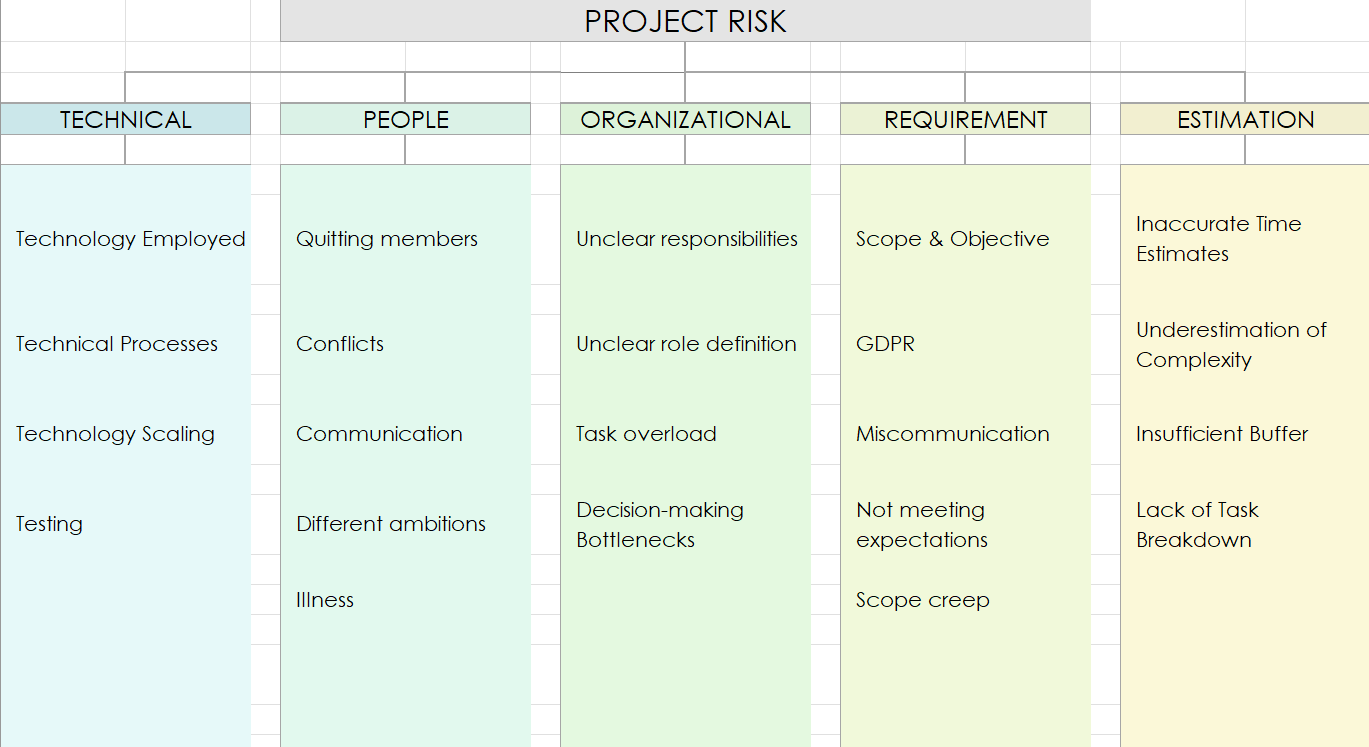
\includegraphics[width=1.0\linewidth]{Risk Diagram List.png}
    \caption{Risk Breakdown Structure}
    \label{fig:enter-label}
\end{figure}
\pagebreak

\section{Risk Description}
The following table provides detailed descriptions of each identified risk, outlining their potential causes and specific impacts on the project to support further analysis and mitigation efforts.

\begin{table}[h]
\centering
\begin{tabularx}{\linewidth}{|l|X|}
\hline
\multicolumn{1}{|c|}{\textit{\textbf{Risks}}} & \multicolumn{1}{c|}{\textit{\textbf{Risks Description}}}                                                   \tabularnewline \hline
 Technology Employed & Dependency on third-party tools that may become deprecated or unsupported.\tabularnewline \hline
 Technical Processes & Risk of losing critical code due to lack of version management.\tabularnewline \hline
 Technology Scaling & Infrastructure might fail to scale effectively under high load or multiple users.\tabularnewline \hline
 Testing & Limitations in testing environments may affect the ability to test all scenarios.\tabularnewline \hline
 Quitting Members & Team members leaving before project completion can cause delays and quality issues.\tabularnewline \hline
 Conflicts & Disagreements among team members can hinder collaboration and productivity.\tabularnewline \hline
 Communication & Poor communication can lead to misunderstandings and project delays.\tabularnewline \hline
 Different Ambitions & Varying levels of commitment and goals among members may lead to disagreements.\tabularnewline \hline
 Unclear Responsibilities & Ambiguity in roles can cause misalignment and missed deadlines.\tabularnewline \hline
 Scope Creep & Uncontrolled addition of features without adjusting timelines or resources.\tabularnewline \hline
 GDPR & Non-compliance with data protection regulations can result in legal issues.\tabularnewline \hline
 Inaccurate Time Estimates & Underestimating time required for tasks can cause missed deadlines.\tabularnewline \hline
 Underestimation of Complexity & Tasks may be simpler than they seem, leading to unexpected development issues.\tabularnewline \hline

\end{tabularx}
\caption{Risks identified in the project.}
\label{table:risks}   
\end{table}
\pagebreak

\section{Risk Analysis}

To evaluate risks, each will be graded on a scale from 1 to 4 for both probability and impact, with 1 representing the lowest and 4 the highest levels. The risk magnitude is then calculated by multiplying the probability by the impact, yielding a risk magnitude indicator ranging from 1 to 16.


IMAGINE A TABLE HERE

\section{Risk Planning}

The Risk Planning details proactive strategies for managing identified risks throughout the project. By implementing these measures, the project aims to minimize potential disruptions and ensure successful outcomes.

IMAGINE ANOTHER TABLE HERE

\section{Risk Monitoring}

Ongoing evaluation and monitoring of risks will be conducted to ensure that mitigation strategies are effective and to address new risks as they emerge throughout the project lifecycle.

IMAGINE A TABLE ABOUT CURRENT RISKS

\end{document}
